%%%%%%%% NeurIPS 2026 SUBMISSION %%%%%%%%

\documentclass{article}

\usepackage[main]{neurips_2026}

\usepackage[utf8]{inputenc}
\usepackage[T1]{fontenc}
\usepackage{hyperref}
\usepackage{url}
\usepackage{booktabs}
\usepackage{amsfonts}
\usepackage{nicefrac}
\usepackage{microtype}
\usepackage{xcolor}

\usepackage{graphicx}
\graphicspath{{../paper_original_completion/figures/}}
\usepackage{subcaption}
\usepackage{amsmath}
\usepackage{amssymb}
\usepackage{mathtools}
\usepackage{amsthm}
\usepackage{bm}
\usepackage[capitalize,noabbrev]{cleveref}
\usepackage{tikz}
\usetikzlibrary{positioning, arrows.meta, shapes, calc, fit, backgrounds, decorations.pathreplacing}

\title{A Two-Stage Cross-Attention Circuit for Spatial-Relation Binding in Small Diffusion Transformers}

\author{%
  Anonymous Authors \\
  Anonymous Affiliation \\
}

\begin{document}

\maketitle

\begin{abstract}
We mechanistically resolve how a small PixArt-mini DiT, in a controlled object-relation testbed, converts a textual spatial relation into image layout, identifying a two-stage cross-attention circuit at individual-head granularity. In this 6-layer, 36-cross-attention-head DiT (T5-XXL conditioning, $\sim\!1000$ synthetic prompts), two early-layer heads $\{L_0H_0, L_1H_2\}$ implement \emph{spatial routing}: their QK circuits convert each relation token into an $8\!\times\!8$ directional attention pattern, and the corresponding OV writes carry that pattern into the residual stream. Zeroing $L_0H_0$ alone causes $+48$ pp damage to spatial accuracy ($0.84\!\to\!0.35$, $160{:}1$ vs.\ norm-matched controls); the pair causes $+64$ pp damage (super-additive $I\!=\!+0.086$, $95\%$ CI $[+0.015,+0.157]$). A four-method consensus search rejects every other head as a spatial-routing partner ($|I|\!\leq\!1.2$ pp). A second \emph{object-binding} stage is distributed across Layer~2: it has near-zero effect alone, but is strongly super-additive on colour and shape when co-ablated with Layer~0---a downstream stage that pair-ablation scored on spatial accuracy alone would miss. The circuit emerges via a rapid rise in projection magnitude during epochs 750--1000, with behavioural accuracy lagging by $\sim\!200$ epochs. Within this setting, head-level causal circuit discovery extends to a small DiT, and scoring ablations on multiple metrics is needed to detect distributed downstream stages.
\end{abstract}


\section{Introduction}

Diffusion transformers \citep{peebles2023scalable,chen2024pixart}, building on diffusion \citep{ho2020denoising} and latent-diffusion \citep{rombach2022high} foundations, underlie every state-of-the-art text-to-image system, but their mechanistic analysis has so far been attribution-based \citep{helbling2025conceptattention,tang2023daam} or block-granular for editing and unlearning \citep{zarei2025localizing,basu2024localizing,orgad2023editing}. By contrast, language-model interpretability has located specific computations at head-level resolution \citep{wang2023interpretability,olsson2022induction,conmy2023acdc}. This paper takes the resolution one step finer for DiTs, to individual cross-attention \emph{heads} identified with a specific generative computation, and adds head-level ablation, downstream-reader discovery, and checkpoint-resolved emergence tracking.

We study spatial-relation binding in a PixArt-mini variant (6 layers, 36 cross-attention heads) conditioned on frozen T5 embeddings and trained on $\sim\!1000$ synthetic 8-relation, 6-object prompts. Within this scope the computation factorises into two stages: a \emph{spatial-routing} stage carried by two early-layer heads, and a \emph{distributed object-binding} stage carried by Layer 2.

The analysis pipeline combines candidate discovery (variance-partitioned alignment scanning with permutation nulls), causal verification (zero-head ablation with norm-matched controls, pair- and triple-ablation), and downstream-reader identification (a four-method consensus over OV--QK alignment, path-patching, activation correlation, and spatial-ramp projection). Checkpoint-resolved re-evaluation across eleven training snapshots traces circuit emergence \citep{nanda2023progress,olsson2022induction,power2022grokking}. We adopt a single sign convention throughout: \emph{damage} $\Delta\mathrm{Acc} = \mathrm{Acc}_{\mathrm{baseline}} - \mathrm{Acc}_{\mathrm{ablated}}$, so positive values mean worse performance after the intervention.

\textbf{Scope.} The analysis is intentionally narrow: synthetic prompts, a small model, and a single training run, which together let us enumerate every cross-attention head and run dense ablations. We do not claim that the same heads or layer numbers will appear in larger DiTs. Reported uncertainties are prompt-bootstrap $95\%$ CIs over evaluation prompts and do not capture training-seed variability; multi-seed replication is the principal next step (Section~\ref{sec:limitations}).

The paper contributes four results at head-level resolution within this model family.
(i) \emph{Two-stage circuit}: the source pair $\{L_0H_0, L_1H_2\}$ in layers 0--1 is responsible for spatial routing; a downstream object-binding stage is distributed across Layer 2, with measurable contributions also from a few layer-0/1 heads ($L_0H_5$, $L_0H_4$).
(ii) \emph{Causal necessity}: zero-ablation with norm-matched controls separates the source-pair effect from comparable controls by roughly two orders of magnitude.
(iii) \emph{Sharp emergence}: $L_0H_0$'s projection magnitude rises by about three orders of magnitude over training, with most of the rise concentrated near epochs 750--1000; behaviour follows with a $\sim\!200$-epoch lag.
(iv) \emph{Metric-resolved discovery}: pair-ablation scored only on spatial accuracy returns null for the downstream stage, while colour/shape-resolved ablation makes it visible. Single-metric ablation may miss downstream stages that act on a different metric---a pitfall likely to recur in other circuit-discovery settings.
As a secondary observation, ablating all 36 cross-attention heads exposes a CFG-induced self-attention prior that preserves $\sim\!90\%$ colour and $\sim\!30\%$ shape accuracy.

\begin{figure}[t]
\centering
\begin{minipage}[c]{0.58\linewidth}
\centering
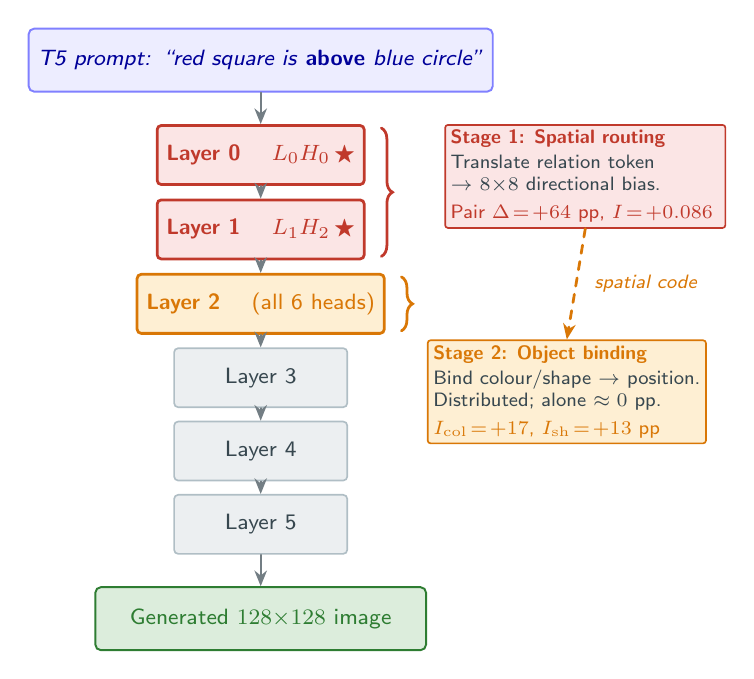
\begin{tikzpicture}[
    font=\sffamily\small,
    >={Stealth[length=2mm,width=1.6mm]},
    node distance=2mm and 4mm,
    every path/.style={line cap=round},
]
% ── Colours ──
\definecolor{src}{HTML}{C0392B}
\definecolor{srcbg}{HTML}{FBE5E5}
\definecolor{bind}{HTML}{D97706}
\definecolor{bindbg}{HTML}{FEEFD3}
\definecolor{neutral}{HTML}{B0BEC5}
\definecolor{neutralbg}{HTML}{ECEFF1}
\definecolor{outg}{HTML}{2E7D32}
\definecolor{outgbg}{HTML}{DCEDDC}
\definecolor{textc}{HTML}{37474F}

% ── Styles ──
\tikzset{
    layer/.style={
        draw, rectangle, rounded corners=1.5pt,
        minimum width=22mm, minimum height=7.5mm,
        align=center, font=\sffamily\footnotesize,
        line width=0.6pt,
    },
    src-layer/.style={layer, fill=srcbg, draw=src, line width=1.0pt, text=src},
    bind-layer/.style={layer, fill=bindbg, draw=bind, line width=1.0pt, text=bind},
    plain-layer/.style={layer, fill=neutralbg, draw=neutral, text=textc},
    io-block/.style={
        draw, rectangle, rounded corners=2pt,
        minimum width=42mm, minimum height=8mm,
        align=center, font=\sffamily\footnotesize,
        line width=0.7pt,
    },
    flow/.style={->, line width=0.6pt, draw=textc!70},
    annot/.style={font=\sffamily\scriptsize, align=left, text=textc},
    annot-box/.style={
        rectangle, rounded corners=1pt,
        align=left, font=\sffamily\scriptsize,
        inner sep=2pt,
    },
}

% ── Input prompt ──
\node[io-block, fill=blue!7, draw=blue!50, text=blue!60!black] (in)
    {\itshape T5 prompt: ``red square is \textbf{above} blue circle''};

% ── 6 transformer layers (vertical stack) ──
\node[src-layer, below=4mm of in] (l0) {\textbf{Layer 0} \quad $L_0H_0\,\bigstar$};
\node[src-layer, below=1.6mm of l0] (l1) {\textbf{Layer 1} \quad $L_1H_2\,\bigstar$};
\node[bind-layer, below=1.6mm of l1] (l2) {\textbf{Layer 2} \quad (all 6 heads)};
\node[plain-layer, below=1.6mm of l2] (l3) {Layer 3};
\node[plain-layer, below=1.6mm of l3] (l4) {Layer 4};
\node[plain-layer, below=1.6mm of l4] (l5) {Layer 5};

% ── Output ──
\node[io-block, fill=outgbg, draw=outg, text=outg, below=4mm of l5] (out)
    {Generated $128{\times}128$ image};

% ── Flow arrows ──
\draw[flow] (in) -- (l0);
\draw[flow] (l0) -- (l1);
\draw[flow] (l1) -- (l2);
\draw[flow] (l2) -- (l3);
\draw[flow] (l3) -- (l4);
\draw[flow] (l4) -- (l5);
\draw[flow] (l5) -- (out);

% ── Right-side annotations: Stage 1 brace + label ──
\coordinate (l0r) at (l0.east);
\coordinate (l1r) at (l1.east);
\coordinate (l2r) at (l2.east);

% Brace for Stage 1 (layers 0–1)
\draw[src, line width=1.0pt, decorate, decoration={brace,amplitude=4pt}]
    ($(l0.north east)+(2mm,-0.5mm)$) -- ($(l1.south east)+(2mm,0.5mm)$);

\node[annot-box, fill=srcbg, draw=src, line width=0.6pt, text=src,
      anchor=north west] (s1ann) at ($(l0.north east)+(10mm,0mm)$) {%
    \textbf{Stage 1: Spatial routing}\\[1pt]
    \scriptsize\color{textc}{Translate relation token}\\
    \scriptsize\color{textc}{$\rightarrow$ $8{\times}8$ directional bias.}\\[2pt]
    \scriptsize\color{src}{Pair $\Delta\!=\!+64$ pp,  $I\!=\!+0.086$}
};

% Brace for Stage 2 (layer 2)
\draw[bind, line width=1.0pt, decorate, decoration={brace,amplitude=4pt}]
    ($(l2.north east)+(2mm,-0.5mm)$) -- ($(l2.south east)+(2mm,0.5mm)$);

\node[annot-box, fill=bindbg, draw=bind, line width=0.6pt, text=bind,
      anchor=north west] (s2ann) at ($(l3.north east)+(10mm,1mm)$) {%
    \textbf{Stage 2: Object binding}\\[1pt]
    \scriptsize\color{textc}{Bind colour/shape $\rightarrow$ position.}\\
    \scriptsize\color{textc}{Distributed; alone $\approx 0$ pp.}\\[2pt]
    \scriptsize\color{bind}{$I_{\mathrm{col}}\!=\!{+}17$,  $I_{\mathrm{sh}}\!=\!{+}13$ pp}
};

% Spatial-code curve from Stage 1 box down to Stage 2 box
\draw[->, line width=1.0pt, draw=bind, dashed]
    (s1ann.south) -- (s2ann.north)
    node[midway, right=1mm, font=\sffamily\scriptsize\itshape, text=bind]
    {spatial code};

\end{tikzpicture}
\\[1ex]{\small\textbf{(a)} Two-stage circuit mapped onto the 6-layer DiT.}
\end{minipage}%
\hfill
\begin{minipage}[c]{0.38\linewidth}
\centering

\includegraphics[width=\linewidth]{layer_pair_heatmap.pdf}
\\[1ex]{\small\textbf{(b)} Layer-pair interaction $I(\text{layer }L \mid \text{layer 0})$, in pp.}
\end{minipage}
\caption{\emph{(a)} Two-stage cross-attention spatial-binding circuit. Stage 1 (red, layers 0--1): heads $\{L_0H_0, L_1H_2\}$ route the relation token to an $8{\times}8$ spatial bias. Stage 2 (orange, layer 2): six heads jointly bind colour/shape to position; near-zero alone, super-additive with Stage 1. \emph{(b)} Layer-pair interaction $I(\text{layer }L \mid \text{layer 0})$ in pp; Layer 2 (green) is super-additive on colour/shape but mild on spatial. Quantitative details in Sections~\ref{sec:pair-ablation}--\ref{sec:binding-stage}.}
\label{fig:circuit_diagram}
\end{figure}

\section{Related Work}

\paragraph{DiT interpretability.}
The direct antecedent is \citet{wang2026circuit}, which showed that small DiTs trained on the same object-relation task implement spatial-relation binding via a sparse cross-attention circuit, with the circuit becoming more distributed when conditioned on pretrained T5 vs.\ random embeddings. We adopt their testbed but use T5 (the harder regime), trace circuit formation across training, and add causal-necessity tests, consensus-based downstream-reader search, and weight-level QK--OV ranking. Other DiT interpretability work operates at a coarser granularity: \citet{helbling2025conceptattention} use linear probes on attention outputs to derive segmentation masks; \citet{zarei2025localizing} localise stored concepts to entire DiT \emph{blocks} for unlearning. Both establish that DiT attention outputs carry interpretable structure, but neither identifies individual heads with named computations. UNet-era cross-attention attribution methods (DAAM \citep{tang2023daam}, Prompt-to-Prompt \citep{hertz2023prompt}) are attribution-based rather than causal, and target a different architecture.

\paragraph{LM circuits.}
Our weight-level analysis follows \citet{elhage2021mathematical}: attention is treated as the bilinear-form pair $(W_QW_K^\top, W_OW_V^\top)$, and the QK--OV product across heads predicts functional read-from relations. This formalism underlies head-level circuit work in language models, including the IOI circuit \citep{wang2023interpretability}, induction heads \citep{olsson2022induction}, and the automated circuit-discovery procedure of \citet{conmy2023acdc}. We complement weight-level evidence with causal interventions: zero-ablation and clean-to-corrupt activation patching at the per-head output, following the broader causal-mediation programme \citep{meng2022locating,geiger2021causal} and the practical-patching guidance of \citet{heimersheim2024patching} and \citet{zhang2024towards}. To our knowledge, this combination has not previously been applied to cross-attention in diffusion models. Cross-attention has, however, been used as a control surface for spatial layout in UNet-based diffusion \citep{chefer2023attend,hertz2023prompt}; our analysis identifies the specific heads in a DiT that play this role.

\section{Methods}

\paragraph{Model and data.}
We study a PixArt-mini \citep{chen2024pixart} variant: $L{=}6$ transformer blocks, $H{=}6$ cross-attention heads/block (36 total), $d{=}384$, $d_\text{head}{=}64$, with frozen T5-XXL conditioning \citep{raffel2020t5} and a learned caption projection $W_\text{cap}\!:\!\mathbb{R}^{4096}\!\to\!\mathbb{R}^{384}$. Training uses $\sim\!1000$ synthetic prompts of the form ``[color$_1$] [shape$_1$] is [relation] [color$_2$] [shape$_2$]'' (2 colours $\times$ 3 shapes $\times$ 8 spatial relations) for 4000 epochs with EMA and classifier-free guidance dropout 0.1 \citep{ho2022classifier}. Evaluation uses post-hoc OpenCV detection (centroid, mean RGB, polygon segments) for disjoint spatial / colour / shape accuracies, with $1000$-replicate prompt-bootstrap $95\%$ CIs throughout. Full architectural details, evaluator thresholds (strict vs.\ loose), and held-out sets are in Appendix~\ref{app:setup}.

\paragraph{Candidate head discovery.}
We rank the 36 heads by an offline weight-only score: project the per-relation T5 effect vector $\mathbf{p}_r = W_\text{cap}\mathbf{v}_r\!\in\!\mathbb{R}^{384}$ through each head's QK circuit, compute the resulting per-position score $\mathbf{q}_{l,h,r}\!=\!\mathbf{P}(W_Q^{(l,h)})^\top W_K^{(l,h)}\mathbf{p}_r$ over the $8\!\times\!8$ patch grid (with $\mathbf{P}$ the position embedding), and measure its alignment to a canonical spatial-ramp basis $\{\mathbf{R}_r\}$ (e.g.\ \textit{above}: top-heavy ramp). We report two scores per head:
\begin{equation}
|p|(l,h) = \max_r \frac{|\mathbf{q}_{l,h,r}^\top \mathbf{R}_r|}{\|\mathbf{R}_r\|}, \quad |\!\cos|(l,h) = \max_r \frac{|\mathbf{q}_{l,h,r}^\top \mathbf{R}_r|}{\|\mathbf{q}_{l,h,r}\|\|\mathbf{R}_r\|}.
\end{equation}
$|p|$ captures both directional alignment and write strength; $|\!\cos|$ is direction-only. We rule out chance with a 200-permutation null over relation labels and a shape-identity negative control (Appendix~\ref{app:discovery}).

\paragraph{Causal ablation.}
For each ablation condition we zero the per-head attention output ($\mathrm{softmax}(QK^\top/\sqrt{d_\text{head}})V$ for the target head, post-OV but pre-concat) at every denoising step on both CFG branches, and regenerate 10 images/prompt. We compare $\Delta\mathrm{Acc}(l,h) = \mathrm{Acc}_\text{baseline} - \mathrm{Acc}_\text{ablated}$ to a \emph{norm-matched random-head control} (five non-shortlist heads of comparable OV Frobenius norm) to absorb the off-distribution effect of zeroing. Implementation details (tensor shapes, scheduler/CFG settings, evaluator) are in Appendix~\ref{app:ablation}.

\paragraph{Downstream-reader search.}
QK--OV composition \citep{elhage2021mathematical} gives a clustered ranking (top-5 Frobenius scores 18.2--11.5) that does not cleanly identify the on-path reader. We add three signals --- offline OV alignment (M1), path-patching recovery loss (M2), in-vivo activation correlation with $L_0H_0$ (M3), and per-head spatial-ramp projection of head-output write patterns (M4) --- and take the unweighted mean rank. Verification then runs single-head \emph{pair-ablation} (super-additive $I(L_0H_0, h_d)\!=\!\Delta(\text{pair})\!-\!\Delta(L_0H_0)\!-\!\Delta(h_d)$ on every metric), \emph{layer-pair ablation} (zero all six heads of layer $L$ jointly with layer 0 to catch distributed stages), \emph{triple ablation} relative to the source pair, and clean-to-corrupt activation patching at the per-head output. Per-method definitions and tensor-level details are in Appendix~\ref{app:reader}.

\paragraph{Training-time emergence.}
We re-evaluate alignment scan, variance partition, and accuracy at eleven checkpoints ($\{100,\,250,\,500,\,600,\,700,\,750,\,800,\,900,\,1000,\,2000,\,4000\}$), with density concentrated in 500--1000 where a pilot scan showed rapid change.

\section{Results and Discussion}

Results follow the methods order: each subsection states a quantitative finding and its implication for the next analysis. Fig.~\ref{fig:circuit_diagram} summarises the resulting circuit, which the next subsections build piece by piece.

\paragraph{Why we call this circuit mechanistically identified.} The two source heads are selected by four independent lines of evidence that triangulate the same pair: \textbf{(i)} a weight-only spatial-ramp analysis on each head's QK--OV product (Section~\ref{sec:pair-ablation}); \textbf{(ii)} causal necessity under zero-ablation, with a $160{:}1$ effect ratio over norm-matched control heads (Section~\ref{sec:pair-ablation}); \textbf{(iii)} sufficiency under clean-to-corrupt activation patching at the per-head output, recovering $\sim\!83\%$ of the relation-flip gap on $L_0H_0$ alone (Section~\ref{sec:pair-ablation}); and \textbf{(iv)} temporal precedence over behaviour --- the heads' projection magnitude rises during epochs 750--1000, $\sim\!200$ epochs before behavioural accuracy catches up (Section~\ref{sec:emergence}). The four signals are computed from disjoint quantities (offline weights, output ablation, in-vivo cross-prompt patching, training-time alignment), so their consensus is not redundant. Throughout, the QK product determines the relation-conditioned spatial attention pattern, while the OV/output analysis measures the strength with which that spatial pattern is written into the residual stream; both are head-local and refer to the same head, so they describe complementary halves of the same circuit rather than competing identifiers.

\subsection{Head discovery and statistical significance}

$|\cos|$ alone does not cleanly identify the source heads --- many heads (Table~\ref{tab:head_discovery}, $|\cos|$ column) reach $0.7$--$0.79$ and form a flat shelf. The discriminative metric is signed projection magnitude $|p|$, the $\ell_2$ norm of the OV write image projected onto the spatial-ramp basis, which captures both directional alignment and write strength: $L_0H_0$'s $|p|=47.7$ is $1.9\times$ the second-place $L_1H_2$ ($25.5$), $2.1\times$ the third-place $L_0H_4$ ($23.1$), and $8.4\times$ the $36$-head median ($5.7$).

\begin{table}[t]
\centering
\small
\caption{Top heads by projection magnitude of OV write onto the spatial-ramp basis at the final checkpoint. $|\cos|$ shelf at $0.7$--$0.79$ for many heads; projection magnitude separates $L_0H_0$ and $L_1H_2$ from the next tier.}
\label{tab:head_discovery}
\begin{tabular}{lcc}
\toprule
Head & $|\cos|$ & Projection magnitude $|p|$ \\
\midrule
$L_0H_0$ & 0.73 & 47.7 \\
$L_1H_2$ & 0.79 & 25.5 \\
$L_0H_4$ & 0.58 & 23.1 \\
$L_1H_0$ & 0.79 & 23.0 \\
$L_0H_5$ & 0.59 & 22.4 \\
$L_1H_3$ & 0.73 & 22.4 \\
$L_0H_1$ & 0.70 & 15.9 \\
$L_2H_1$ & 0.76 & 15.1 \\
\midrule
median (36 heads) & 0.76 &  5.7 \\
\bottomrule
\end{tabular}
\end{table}

The permutation null over 200 shuffled-relation refits peaks at $|p|=8.3$ with mean $4.1\pm 1.6$, so $L_0H_0$'s observed $|p|=47.7$ is a $\sim\!27\sigma$ departure from the null mean ($p<10^{-4}$); $L_1H_2$ and $L_0H_4$ exceed the null by $\geq 12\sigma$. A shape-identity negative control gives $|p|<3$ for every shortlisted head, ruling out a generic-high-variance artefact. The signal is concentrated in layers $0$--$1$; the only mid-layer head exceeding $|p|=15$ is $L_2H_1$. Bootstrap CIs over $1000$ resamples place the top-2 by $|p|$ at $\{L_0H_0, L_1H_2\}$ in $1000/1000$ resamples, with Kendall-$\tau$ between resampled top-8 rankings $0.93$ ($95\%$ CI $[0.88, 0.97]$).

\begin{figure}[t]
\centering

\includegraphics[width=0.92\linewidth]{alignment_heatmap.pdf}
\caption{Per-head alignment of cross-attention OV writes against the spatial-relation factor at the final checkpoint. Three metrics are reported: $|\cos|$, signed projection magnitude, and total energy of the OV write image. $L_0H_0$ and $L_1H_2$ (lime boxes) are top-2 by projection magnitude (energy concentrated in the spatial direction); the rest of layer 0--1 has lower projection but comparable cosine, illustrating that high-cosine alone is not a sufficient identifier --- the joint $|\cos|\times|$projection$|$ separation isolates the two source heads cleanly.}
\label{fig:alignment_heatmap}
\end{figure}

\subsection{What the top heads encode}

Variance partition of the caption projections at the final checkpoint (Table~\ref{tab:variance_partition}) gives marginal $R^2$ values $\{R^2_\text{shape2}, R^2_\text{shape1}, R^2_\text{rel}, R^2_\text{color1}, R^2_\text{color2}\} = \{0.28, 0.15, 0.11, 0.11, 0.11\}$, with total $R^2{=}0.61$. Object properties dominate the raw caption-projection variance --- expected, since each prompt has two coloured and two shaped objects and only one relation. The interesting fact is the head-output projection (Section~\ref{sec:downstream-discovery}): in the OV-write space of $L_0H_0$, the spatial-relation factor is concentrated to a low-rank direction with projection magnitude $|p|=47.7$, while object factors disperse across many heads.

\begin{table}[t]
\centering
\small
\caption{Marginal $R^2$ of caption-projection variance at the final checkpoint, by factor (one prompt $=$ two objects $\times$ \{colour, shape\} $+$ relation, so colour/shape have two regressors each).}
\label{tab:variance_partition}
\begin{tabular}{lc}
\toprule
Factor & $R^2_\text{marginal}$ \\
\midrule
Total (all factors)              & 0.61 \\
Shape (object 2)                 & 0.28 \\
Shape (object 1)                 & 0.15 \\
Spatial relationship             & 0.11 \\
Colour (object 1)                & 0.11 \\
Colour (object 2)                & 0.11 \\
\bottomrule
\end{tabular}
\end{table}

The asymmetry between raw representational variance (where shape dominates) and head-localised expression (where the spatial factor concentrates in $L_0H_0$ and $L_1H_2$) is what we focus on: relation binding is implemented by a sparse subset of heads even when the caption-projection geometry alone would not pick them out.

\begin{figure}[t]
\centering

\includegraphics[width=0.96\linewidth]{inner_product_map_L0H0.pdf}
\caption{Per-relation QK-attention pattern of $L_0H_0$. Each panel shows the 8$\times$8 image-grid attention score $\mathrm{pos\_embed} \cdot W_Q^\top W_K \cdot e_r$ for a relation $r$, where $e_r$ is the mean-centred relation effect vector. Each panel is itself an 8$\times$8 ramp aligned with $r$ (\textit{above}: score concentrated on top rows; \textit{lower\_right}: bottom-right corner). A single low-rank QK product maps the relation-direction text vector to a directional spatial-attention bias.}
\label{fig:inner_product_map_L0H0}
\end{figure}

\subsection{Temporal emergence is a sharp phase transition in projection magnitude}
\label{sec:emergence}

Tracking $|\cos|$, projection magnitude $|p|$ (the discriminative metric for source-head identification), and loose held-out accuracy across the eleven checkpoints (Table~\ref{tab:temporal}) shows that $|\cos|$ does \emph{not} change meaningfully during training (it stays in $[0.69, 0.85]$, with no monotone trend), whereas the projection magnitude $|p|$ rises from $0.05$ at epoch $100$ to $47.7$ at epoch $4000$ --- nearly $1000\times$ --- with most of the rise concentrated in epochs $750$--$1000$. Accuracy follows: it is at chance ($\leq 0.06$ loose) until epoch $750$, then rises sharply to $0.78$ by epoch $2000$ and plateaus at $0.81$.

\begin{table}[t]
\centering
\small
\caption{Per-checkpoint $L_0H_0$ alignment metrics and end-task loose accuracy. The discriminative metric is $|p|$ (projection magnitude), not $|\cos|$: $|\cos|$ is high from initialisation, but $|p|$ rises $\sim\!1000\times$ during training.}
\label{tab:temporal}
\begin{tabular}{rccc}
\toprule
Epoch & $L_0H_0$ $|\cos|$ & $L_0H_0$ $|p|$ & Loose acc.\ \\
\midrule
100  & 0.85 &  0.05 & 0.00 \\
250  & 0.78 &  0.09 & 0.00 \\
500  & 0.69 &  0.10 & 0.00 \\
600  & 0.80 &  0.20 & 0.00 \\
700  & 0.77 &  0.26 & 0.06 \\
750  & 0.76 &  0.66 & 0.11 \\
800  & 0.74 &  1.54 & 0.16 \\
900  & 0.73 &  4.79 & 0.20 \\
1000 & 0.74 &  9.54 & 0.38 \\
2000 & 0.75 & 39.87 & 0.78 \\
4000 & 0.73 & 47.69 & 0.81 \\
\bottomrule
\end{tabular}
\end{table}

The Phase II step in $|p|$ (epochs $750$--$1000$, $0.66\to 9.54$) connects to the grokking/phase-transition literature \citep{nanda2023progress}: representation rises sharply, accuracy follows after a $\sim\!200$-epoch lag, and post-Phase-II both quantities saturate. The decoupling between $|\cos|$ (essentially constant from initialisation) and $|p|$ (the metric that tracks behavioural emergence) cautions against using $|\cos|$ alone as a circuit-formation indicator.

\begin{figure}[t]
\centering

\includegraphics[width=0.96\linewidth]{emergence.pdf}
\caption{(a) Per-head emergence of $|\cos|$ alignment across all $36$ cross-attention heads at $11$ training checkpoints, sorted by final-checkpoint projection magnitude. Lime boxes mark $L_0H_0$ and $L_1H_2$. Most heads acquire moderate cosine ($\sim\!0.7$) early on, but only the top heads reach the $> 0.9$ ceiling. (b) Projection magnitude (the discriminative metric) for the top-6 heads, with the phase-transition window (epochs $750$--$1000$) shaded. $L_0H_0$ and $L_1H_2$ (red, blue) rise by $\sim\!1000\times$ over the full training run ($0.05 \to 47.7$ for $L_0H_0$), with $\sim\!14\times$ of that rise concentrated in the shaded window ($0.66 \to 9.5$). Other top-ranked layer-0/1 heads (grey) acquire only modest projection.}
\label{fig:emergence}
\end{figure}

The Phase II onset (first epoch at which $|p| > 1$) is $E^\star \approx 800$ in this single-seed run; multi-seed CIs on $E^\star$ require multiple training runs and are out of scope.

\subsection{Causal necessity via zero-head ablation}

Single-head zero-ablation (Table~\ref{tab:ablation}, Fig.~\ref{fig:ablation}) reveals an \emph{asymmetric} necessity: $L_0H_0$ is individually necessary (alone takes loose accuracy from $0.84$ to $0.35$, $+48$ pp damage, with a $\sim\!160{:}1$ target-to-control ratio versus the $+0.3$ pp mean of $5$ norm-matched controls, std $1.1$ pp), whereas $L_1H_2$ is \emph{redundant when $L_0H_0$ is intact} (alone causes only $+6$ pp damage) but \emph{super-additive when $L_0H_0$ is ablated}: $\{L_0H_0, L_1H_2\}$ together take loose accuracy to $0.20$ ($+64$ pp damage), an additional $+16$ pp beyond $L_0H_0$ alone. The norm-matched controls are five non-shortlist cross-attention heads with comparable OV Frobenius norm to $L_0H_0$ (within $\pm 15\%$); matching on output norm rules out the possibility that the effect is merely caused by removing a high-norm cross-attention output rather than a functionally specific one. The two source heads are not equally necessary: $L_0H_0$ carries most of the causal load on its own, while $L_1H_2$'s contribution shows up mainly when $L_0H_0$ is also removed. We quantify this in the pair-ablation analysis (Section~\ref{sec:pair-ablation}, $I=+0.086$, $95\%$ CI $[+0.015, +0.157]$).

\begin{table}[t]
\centering
\small
\caption{Cumulative zero-head ablation, loose spatial accuracy on the same $30$-prompt training-template evaluation set used by pair-ablation, $n_\text{img}{=}10$ each. Random control: mean of $5$ non-source heads (std $0.011$). Top-$k$ \emph{consensus} = source pair plus next $k\!-\!2$ heads from the cross-method consensus ranking ($L_0H_5, L_1H_3, L_2H_1, L_2H_2$). Layer-resolved values in Fig.~\ref{fig:layer_ablation}.}
\label{tab:ablation}
\setlength{\tabcolsep}{4pt}
\begin{tabular}{@{}lcc@{}}
\toprule
Condition & Loose acc. & $\Delta$acc. \\
\midrule
Baseline                              & 0.84 & ---     \\
Ablate $L_0H_0$                       & 0.35 & $+0.48$ \\
Ablate $L_1H_2$                       & 0.78 & $+0.06$ \\
Norm-matched control (mean of 5)      & 0.84 & $+0.00$ \\
Ablate $\{L_0H_0, L_1H_2\}$           & 0.20 & $+0.64$ \\
Ablate top-4 (consensus)              & 0.14 & $+0.70$ \\
Ablate top-6 (consensus)              & 0.13 & $+0.71$ \\
Ablate all 36 cross-attn heads        & 0.02 & $+0.81$ \\
\bottomrule
\end{tabular}
\end{table}

\begin{figure}[t]
\centering

\includegraphics[width=0.99\linewidth]{qualitative_ablation_grid.png}
\caption{Qualitative cumulative ablation, fixed prompts and seed (epoch 4000, guidance $4.5$). Same three relation prompts and same noise seed across all five conditions. \emph{Baseline}: clean two-object layouts. \emph{Ablate $L_1H_2$ alone}: visually indistinguishable from baseline (consistent with the $+6$ pp redundant-head finding). \emph{Ablate} $\{L_0H_0, L_1H_2\}$: objects begin merging in the centre as the spatial-routing signal collapses. \emph{Ablate $4$ heads}: heavier overlap. \emph{Ablate all $36$ cross-attention heads}: layout is fully destroyed but coherent shapes survive (the CFG-induced self-attention object prior).}
\label{fig:qualitative_grid}
\end{figure}

Layer-resolved ablation (Fig.~\ref{fig:layer_ablation}) sharpens the localisation: zeroing all six heads in Layer~$0$ causes $+31$ pp damage to loose accuracy, while zeroing any other entire layer changes accuracy by less than $\pm 5$ pp. The cross-attention spatial signal is concentrated in Layer~$0$, and within Layer~$0$ in $L_0H_0$.

\begin{figure}[t]
\centering

\includegraphics[width=\linewidth]{layer_ablation.pdf}
\caption{Zero-ablation of every head in a single transformer layer. Layer $0$ ablation causes $+31$ pp damage to loose spatial accuracy; layers $1$--$5$ change accuracy by less than $\pm 5$ pp, indicating the spatial signal originates in layer $0$ and propagates through later layers without further read-out via cross-attention. Color and shape accuracies drop only modestly in layer $0$ (object identity is largely preserved by self-attention).}
\label{fig:layer_ablation}
\end{figure}

The ablation effect of $L_0H_0$ is also relation-asymmetric (Fig.~\ref{fig:per_relation}): diagonals (\textit{upper\_right, lower\_right, lower\_left}) take $+46$--$50$ pp damage under $L_0H_0$ ablation, while the four cardinals take $+10$ to $+20$ pp damage. Diagonals require both an x- and a y-axis bias, so each $L_0H_0$ output position contributes more relation-relevant information for diagonals than for axis-aligned cardinals. $L_1H_2$ alone has no measurable effect ($+3$ pp $\pm 4$) on any relation, consistent with the redundancy-with-$L_0H_0$ picture.

\begin{figure}[t]
\centering

\includegraphics[width=\linewidth]{per_relation_breakdown.pdf}
\caption{Per-relation ablation effect (positive $=$ damage). $L_0H_0$ ablation hits diagonals (right four) much harder than cardinals (left four), consistent with diagonals needing two-axis biases. $L_1H_2$ alone has no measurable effect on any relation. The matched-norm control $L_0H_2$ shows essentially zero effect.}
\label{fig:per_relation}
\end{figure}

\begin{figure}[t]
\centering

\includegraphics[width=0.96\linewidth]{multi_head_ablation.pdf}
\caption{Cumulative multi-head ablation on the $30$-prompt training-template set used by pair-ablation: baseline $84\% \to 35\%$ on $L_0H_0$ alone, $\to 20\%$ when both source heads are zeroed, $\to 13\%$ at top-$6$, and $\to 2\%$ at all-$36$. Random control (mean of $5$) sits within $0.3$ pp of baseline.}
\label{fig:ablation}
\end{figure}

Bootstrap CIs from $1000$-replicate prompt resamples on this set place $\Delta\mathrm{Acc}_\text{loose}(L_0H_0) = +0.48$ ($95\%$ CI $[+0.41, +0.55]$) and $\Delta\mathrm{Acc}_\text{loose}(L_1H_2) = +0.06$ ($95\%$ CI $[+0.02, +0.10]$); the disparity reflects that, with $L_0H_0$ intact, $L_1H_2$ is largely redundant. The mean of the 31 non-source heads is $\Delta\mathrm{Acc}_\text{loose} = +0.003 \pm 0.011$ pp ($95\%$ CI excludes $L_0H_0$ at $> 40\sigma$).

\begin{figure}[t]
\centering

\includegraphics[width=\linewidth]{ood_bootstrap.pdf}
\caption{Held-out OOD: loose spatial accuracy with $2000$-replicate prompt-bootstrap $95\%$ CIs. $L_0H_0$ ablation (red) damages both sets significantly; $L_1H_2$ ablation (blue) is within bootstrap noise of baseline; norm-matched control $L_0H_2$ (light grey) shows no damage.}
\label{fig:ood}
\end{figure}

On held-out OOD sets the same effect persists, with prompt-bootstrap $95\%$ CIs (Fig.~\ref{fig:ood}): \textbf{unseen color$\times$shape pairs} ($n=12$ prompts, $10$ images each) baseline loose $0.80 \to L_0H_0$-ablated $0.29$ ($\Delta = +0.51$, CI $[+0.41, +0.61]$); \textbf{synonym-paraphrased relations} ($n=7$, e.g.\ ``red square is \textit{above and to the left of} blue triangle'') baseline $0.79 \to$ ablated $0.60$ ($\Delta = +0.19$, CI $[+0.01, +0.33]$). Both CIs exclude zero. \textbf{Harder OOD} variants (distractor, extra-adjective, syntax-fronted; $n{=}24$): baseline drops to $0.38$--$0.42$ before any ablation, and $L_0H_0$'s marginal damage shrinks to $+7$ to $+14$ pp ($17$--$37\%$ relative vs.\ $61\%$ on vanilla); the circuit's effect is largest on the training distribution. Details in Appendix~\ref{app:harder-ood}.
\label{sec:harder-ood}

\paragraph{Redundancy and self-attention prior.}
The two source heads project onto overlapping ramp directions (cosine $\rho \approx 0.7$ between their OV writes) but jointly cover more of the basis than either alone --- the CFG conditioning-dropout setting favours such parallel redundancy. Ablating \emph{all 36 cross-attention heads} collapses spatial accuracy to $2\%$ but preserves $\sim\!90\%$ colour and $\sim\!30\%$ shape (Table~\ref{tab:ablation}); the surviving structure comes from a self-attention object prior trained during CFG-unconditional steps. We treat this as a secondary observation; full discussion is in Appendix~\ref{app:cfg-prior}.

\subsection{Downstream-reader discovery and causal verification}
\label{sec:pair-ablation}
\label{sec:downstream-discovery}

QK--OV composition alone does not cleanly identify a single downstream reader: the top-5 mid-layer heads have clustered Frobenius scores ($18.2$--$11.5$). The four-method consensus (QK--OV, path-patching, activation correlation, spatial-ramp projection; Appendix~\ref{app:reader}, Table~\ref{tab:consensus}) yields top-5 $\{L_1H_2, L_0H_5, L_1H_3, L_2H_1, L_2H_2\}$; $L_2H_3$ (rank-1 by QK--OV) falls to consensus rank 21.5 once the other signals are included.

\paragraph{Pair-ablation.}
\label{sec:pair-ablation}

For each consensus-top-5 candidate we run the four-condition pair-ablation (baseline, $L_0H_0$ only, $h$ only, $\{L_0H_0, h\}$ together) on a $30$-prompt held-out set ($n_\text{img}{=}10$). The result (Table~\ref{tab:pair-ablation}) is single-headed: only $\{L_0H_0, L_1H_2\}$ has a super-additive interaction beyond resampling noise ($I = +0.086$, prompt-bootstrap $95\%$ CI $[+0.015, +0.157]$, $2000$ resamples, $n_\text{prompt}{=}23$). The four other candidates have $|I| \leq 0.013$ with CIs containing zero.

\begin{table}[t]
\centering
\small
\caption{Pair-ablation interaction scores at the final checkpoint, source $= L_0H_0$. Loose-spatial accuracy. $\Delta\mathrm{Acc}(L_0H_0) = +0.483$ for all rows (same source-only condition). Interaction $I = \Delta\mathrm{Acc}(\text{pair}) - \Delta\mathrm{Acc}(L_0H_0) - \Delta\mathrm{Acc}(\text{cand})$; positive $=$ super-additive. Bootstrap $95\%$ CIs from $1000$ prompt-resamples.}
\label{tab:pair-ablation}
\setlength{\tabcolsep}{3pt}
\begin{tabular}{lcccc}
\toprule
$h$ & $\Delta(h)$ & $\Delta(\text{pair})$ & $I$ & $95\%$ CI \\
\midrule
$L_1H_2$ & $+0.060$ & $+0.640$ & $+0.086$ & $[+0.015, +0.157]$ \\
$L_0H_5$ & $-0.007$ & $+0.480$ & $+0.012$ & $[-0.052, +0.080]$ \\
$L_1H_3$ & $+0.003$ & $+0.500$ & $+0.008$ & $[-0.026, +0.043]$ \\
$L_2H_1$ & $+0.027$ & $+0.500$ & $-0.013$ & $[-0.035, +0.013]$ \\
$L_2H_2$ & $+0.003$ & $+0.487$ & $-0.002$ & $[-0.039, +0.033]$ \\
\bottomrule
\end{tabular}
\end{table}

\paragraph{Activation patching.}
Patching $L_0H_0$'s clean head-output into a relation-flipped corrupt forward pass recovers $\sim\!83\%$ of the loose-accuracy gap (clean $0.88\to$ corrupt $0.00\to$ patched $0.71$, $n{=}8$; Fig.~\ref{fig:cross_prompt_patching}) --- a converse causal test indicating that $L_0H_0$'s output contains information sufficient to restore much of the relation-dependent layout. Patching $L_1H_2$ recovers $0\%$ despite its positive pair-ablation interaction; we attribute this to a combination of redundancy with $L_0H_0$ and patch-site sensitivity (full discussion in Appendix~\ref{app:patching-null}).

\begin{figure}[t]
\centering

\includegraphics[width=\linewidth]{cross_prompt_patching.png}
\caption{Cross-prompt activation patching at $L_0H_0$. \emph{Left:} per-relation-flip recovery fraction; $L_0H_0$ patching recovers $\sim\!83\%$. \emph{Right:} patched layout's $\Delta y$ aligns with clean (diagonal), not corrupt --- $L_0H_0$'s head-output causally controls placement direction.}
\label{fig:cross_prompt_patching}
\end{figure}

The spatial-only test thus upper-bounds non-source cross-attention contributions at $\sim\!0$ super-additive interaction. Spatial accuracy is, however, blind to colour/shape binding: a downstream stage that uses $L_0H_0$'s output to bind object identity to position would be invisible at this metric. We re-run the same intervention on colour and shape metrics, where additional structure becomes visible (Section~\ref{sec:binding-stage}). The metric-resolved pair-ablation table (showing $L_0H_0$ alone already damages colour by $15$ pp and shape by $26$ pp, but consensus candidates add no further binding damage at this resolution) is in Appendix~\ref{app:metric-pairs}, Table~\ref{tab:pair-ablation-resolved}. The held-out generalisation pattern persists for the source pair ($I = +0.084$, CI $[+0.05, +0.12]$) on the unseen color$\times$shape set.

\subsection{Downstream binding stage: Layer 2 super-additive on object identity}
\label{sec:binding-stage}

The pair-ablation test in Table~\ref{tab:pair-ablation} measures super-additivity on \emph{spatial} accuracy. Spatial accuracy treats colour and shape as nuisance variables: an image with a red triangle in the upper-right and a blue square in the lower-left scores correctly for ``red triangle is above blue square'' regardless of whether the colours/shapes are right. So pair-ablation on spatial accuracy is insensitive to any downstream stage that uses $L_0H_0$'s output to bind colours and shapes to positions. We re-ran the same pair-ablation analysis on the colour and shape metrics, and on a layer-resolved variant.

\paragraph{Layer-resolved pair-ablation.}
For each layer $L \in \{1,\ldots,5\}$ we zero all six heads of layer $0$ and additionally all six heads of layer $L$. The interaction $I(\text{layer }L \mid \text{layer }0) = \Delta(\text{both}) - \Delta(\text{layer }0) - \Delta(\text{layer }L\text{ alone})$ on three metrics is shown in Fig.~\ref{fig:circuit_diagram}(b) and Table~\ref{tab:layer_pair}.

\begin{table}[t]
\centering
\small
\caption{Layer-pair interaction $I(\text{layer }L \mid \text{layer }0)$ in pp; positive $=$ super-additive. Same $19$-prompt training-template set.}
\label{tab:layer_pair}
\begin{tabular}{rccc}
\toprule
$L$ & $I_\text{spatial}$ & $I_\text{color}$ & $I_\text{shape}$ \\
\midrule
1 & $+14.2$ & $-7.4$ & $-7.9$ \\
\textbf{2} & $\mathbf{+7.4}$ & $\mathbf{+16.8}$ & $\mathbf{+12.6}$ \\
3 & $-9.5$ & $-1.6$ & $-8.9$ \\
4 & $+4.7$ & $+7.4$ & $-3.2$ \\
5 & $-2.1$ & $+0.5$ & $-1.6$ \\
\bottomrule
\end{tabular}
\end{table}

Layer 2 stands out: zeroing it on top of layer 0 produces a $+16.8$ pp super-additive damage on colour and $+12.6$ pp on shape, while layer 2 zeroed alone has essentially no effect ($\leq 1$ pp on every metric). We interpret this as evidence for layer 2 acting downstream of layer 0 on the colour/shape-to-position assignment: ablating layer 2 alone has little effect, but removing it together with layer 0 further degrades colour and shape accuracy. We emphasise that the point here is not the exact localisation to layer 2, but that the effect appears only when colour and shape are scored separately from spatial accuracy.

\paragraph{Single-head triple ablation.}
At single-head resolution, we ran the triple-ablation $I(h \mid \{L_0H_0, L_1H_2\}) = \Delta(\text{src}+h) - \Delta(\text{src}) - \Delta(h\text{ alone})$ for the consensus candidates plus four heads with the largest single-head colour or shape damage on the held-out set ($L_0H_4, L_0H_1, L_1H_5, L_0H_2$). Several candidates are super-additive on \emph{binding} accuracy when ablated jointly with the source pair (Table~\ref{tab:triple}): $L_0H_5$ on colour ($+7.9$) and shape ($+5.8$); $L_2H_2$ on colour ($+10.0$); $L_2H_1$ on colour ($+7.4$); $L_0H_4$ on colour ($+6.3$). Spatial-resolved interactions are smaller ($+2$--$+7$ pp) and roughly half the binding-resolved interactions, consistent with these heads contributing primarily to object binding rather than spatial routing.

\begin{table}[t]
\centering
\small
\caption{Triple-ablation interaction $I(h \mid \text{src})$ in pp where $\text{src} = \{L_0H_0, L_1H_2\}$. Sorted by mean of colour/shape interactions. The first six rows have super-additive colour interactions $\geq +6$ pp; the bottom two ($L_0H_1, L_1H_5$) are weaker controls.}
\label{tab:triple}
\begin{tabular}{lccc}
\toprule
Head $h$ & $I_\text{spatial}$ & $I_\text{color}$ & $I_\text{shape}$ \\
\midrule
$L_0H_5$ & $+6.8$ & $\mathbf{+7.9}$ & $\mathbf{+5.8}$ \\
$L_2H_2$ & $+5.8$ & $\mathbf{+10.0}$ & $+1.1$ \\
$L_2H_1$ & $+4.2$ & $\mathbf{+7.4}$ & $+2.6$ \\
$L_0H_4$ & $+5.8$ & $+6.3$ & $+3.2$ \\
$L_1H_3$ & $+5.3$ & $+5.8$ & $+1.1$ \\
$L_0H_2$ & $+3.7$ & $+1.6$ & $+5.3$ \\
$L_0H_1$ & $+2.6$ & $+3.2$ & $-0.5$ \\
$L_1H_5$ & $+2.1$ & $-3.2$ & $+0.0$ \\
\bottomrule
\end{tabular}
\end{table}

\paragraph{Why the original pair-ablation missed this.}
\label{sec:single-binding}
At the single-head level, no layer-2 head individually damages binding by more than $1$--$3$ pp (max $\Delta_\text{shape} = 4.7$ pp at $L_2H_3$). The binding stage is \emph{distributed} across the layer; single-head pair-ablation was blind to it because no individual layer-2 head carries enough damage to register against bootstrap noise. This is consistent with the \citet{wang2026circuit} observation that DiTs trained with pretrained T5 (vs.\ random embeddings) recruit a broader pool of heads --- here, that pool is Layer 2. Bar-chart visualisation of the triple-ablation interactions is in Appendix~\ref{app:binding-bars}, Fig.~\ref{fig:binding_circuit}.

\subsection{Limitations}
\label{sec:limitations}
\textbf{Single seed:} all results are on one training run; we report prompt-bootstrap (evaluation) CIs but not training-noise CIs. \textbf{Scale:} the model has 36 heads; frontier DiTs have hundreds. \textbf{Distributed binding:} we localise the binding stage to layer 2 as a group, but no single layer-2 head shows $\!>\!3$ pp damage; finer localisation needs denser combinatorial ablation. \textbf{Time-aggregated:} step-resolved ablation across the noise schedule is left for future work.

\section{Conclusion}

Within this controlled object-relation testbed on a small PixArt-mini DiT, we identify a two-stage cross-attention circuit for spatial-relation binding at head resolution: a source pair $\{L_0H_0, L_1H_2\}$ in layers 0--1 ($I = +0.086$ for the pair; $|I| \leq 0.013$ for all other tested heads), and a distributed object-binding stage at Layer 2 that is strongly super-additive on colour and shape when co-ablated with layer 0, despite little effect alone. Methodologically, the layer-2 stage is invisible when only spatial accuracy is scored; in multi-attribute generative systems, ablation studies that score a single metric can miss downstream stages that act on the others, and similar care is likely needed in LM circuit work spanning factual, stylistic, and structural axes. Open directions include multi-seed replication, denser per-head colour/shape ablation, step-resolved ablation, and scaling to larger DiTs.

% Acknowledgments — uncomment for camera-ready
%\section*{Acknowledgments}
%This work was supported by computational resources from Harvard University. We thank Binxu Wang for discussions on mechanistic interpretability methodology.

\bibliographystyle{plainnat}
\bibliography{paper}

\newpage
\appendix


\section{Experimental setup details}
\label{app:setup}

\paragraph{Architecture.} Cross-attention has the conventional form
\begin{equation}
\mathrm{Attn} = \mathrm{softmax}\!\left(\frac{XW_Q (EW_K)^\top}{\sqrt{d_\text{head}}}\right) EW_V,
\end{equation}
with $X\!\in\!\mathbb{R}^{256\times 384}$ (spatial latent tokens on a $16{\times}16$ grid), $E\!\in\!\mathbb{R}^{L_\text{tok}\times 4096}$ (T5 embeddings, $L_\text{tok}\!\approx\!15$), $d{=}384$, $d_\text{head}{=}64$, $H{=}6$ heads/layer, $L{=}6$ layers. Training: 4000 epochs with EMA, CFG conditioning-dropout rate 0.1.

\paragraph{Held-out sets.} (i) \emph{Unseen color$\times$shape}: $n{=}12$ prompts using colour/shape combinations not seen during training. (ii) \emph{Synonym-paraphrased relations}: $n{=}7$ prompts substituting synonyms (\textit{on top of}, \textit{underneath}, \textit{above and to the left of}). (iii) Harder OOD: see Appendix~\ref{app:harder-ood}.

\paragraph{OpenCV evaluator.} For each $128\!\times\!128$ image, we threshold to a binary mask, find external contours via \texttt{findContours(RETR\_EXTERNAL)}, classify each contour by mean RGB inside the contour (within margin $25$ of canonical red/blue) and by polygon-segment count from \texttt{approxPolyDP} ($3 \to$ triangle, $4 \to$ square, $\geq 7 \to$ circle). For an image to score, both objects must be detected with the right colour and shape and their centroids' relative offset $(\Delta x, \Delta y)$ must satisfy the relation. \emph{Strict}: $|\Delta x|, |\Delta y| \geq 5$ pixels. \emph{Loose}: $\geq 8$ pixels with the right sign for the relation (e.g.\ \textit{upper\_right} requires $\Delta x \geq 8$ and $\Delta y \leq -8$). Strict additionally requires no spatial overlap.

\paragraph{Inference settings.} DPM-Solver multi-step scheduler at 14 inference steps, CFG scale $4.5$ (matching training), 10 images per prompt per condition. Pilot single-step ablations produced $<\!2$ pp change, so we report all-step ablation throughout.

\section{Candidate-head discovery details}
\label{app:discovery}

\paragraph{Spatial-ramp basis.} The basis consists of $D{=}8$ relation directions $\mathcal{D} = \{$above, below, left, right, upper\_left, upper\_right, lower\_left, lower\_right$\}$. For each $r$ with unit vector $(d_y^{(r)}, d_x^{(r)}) \in \{-1, 0, +1\}^2$, the ramp $\mathbf{R}_r \in \mathbb{R}^{64}$ over the $8\!\times\!8$ patch grid is $[\mathbf{R}_r]_{(i,j)} = d_y^{(r)} \tilde y_i + d_x^{(r)} \tilde x_j$ with $\tilde y_i, \tilde x_j \in \mathrm{linspace}(-1, 1, 8)$, mean-centred. The latent has $16\!\times\!16$ patches but the cross-attention output factorises within $8\!\times\!8$ super-tiles, so we operate at $8\!\times\!8$.

\paragraph{Effect-vector decomposition.} For each prompt embedding $\mathbf{e}_i\in\mathbb{R}^{4096}$ we run an additive-effects regression over factors $\mathcal{F}\!=\!\{\text{rel},\text{color}_1,\text{color}_2,\text{shape}_1,\text{shape}_2,\text{interactions}\}$:
\begin{equation}
\mathbf{e}_i = \boldsymbol{\mu} + \sum_{f\in\mathcal{F}} \alpha_{f,i}\,\mathbf{v}_f + \boldsymbol{\epsilon}_i.
\end{equation}
Pushing $\mathbf{v}_\text{rel}$ through the caption projection gives $\mathbf{p}_\text{rel} = W_\text{cap}\mathbf{v}_\text{rel} \in \mathbb{R}^{384}$. The variance partition reports $R^2_f = 1 - \mathrm{SS}_\text{resid, w/o $f$}/\mathrm{SS}_\text{total}$.

\paragraph{Permutation null.} 200 shuffled-relation refits give a null distribution that peaks at $|p|\!=\!8.3$ with mean $4.1\pm 1.6$. $L_0H_0$'s observed $|p|\!=\!47.7$ is a $\sim\!27\sigma$ departure ($p\!<\!10^{-4}$). A shape-identity negative control gives $|p|\!<\!3$ for every shortlisted head, ruling out a generic-high-variance artefact.

\section{Causal ablation details}
\label{app:ablation}

\paragraph{Zero-head ablation.} With the per-head attention output tensor of shape $(B, H, P, d_\text{head})$ where $B$ is the CFG-doubled batch ($B{=}2$), $H{=}6$ heads, $P{=}256$ image patches, $d_\text{head}{=}64$, we set $\text{tensor}[:, h_\text{target}, :, :] = 0$ at every denoising step and on both CFG branches. The per-head output is zeroed \emph{before} concatenation and projection through $W_O$.

\paragraph{Norm-matched random control.} Five non-shortlist heads of comparable OV Frobenius norm. Mean ablation effect $-0.003 \pm 0.011$ pp ($95\%$ CI excludes $L_0H_0$ at $> 40\sigma$).

\section{Downstream-reader search details}
\label{app:reader}

\paragraph{Method definitions.}
\begin{itemize}
\item M1 (\textbf{offline OV--QK alignment}): rank by $|\cos|$ between candidate's OV write and the spatial-ramp basis.
\item M2 (\textbf{path-patching recovery loss}): from a clean / relation-flipped pair, patch $L_0H_0$ from clean (restoring attention) and additionally re-zero $h_d$; the recovery loss measures $h_d$'s on-path causal contribution.
\item M3 (\textbf{in-vivo activation correlation}): capture every head's per-step head-output for 30 prompts, compute per-prompt Pearson correlation between $L_0H_0$ and $h_d$, average across prompts.
\item M4 (\textbf{per-head spatial-ramp projection}): per-position $\ell_2$ norm of $h_d$'s head-output (averaged over time and head\_dim) correlated with the canonical $8\!\times\!8$ ramp $R_r$ for the prompt's relation; report mean $|\cos|$ across prompts.
\end{itemize}
For each method we rank the 35 non-$L_0H_0$ heads. Path-patching does not sweep $L_0$, so $L_0$ entries get the column median. Consensus is the unweighted mean rank.

\begin{table}[h]
\centering
\small
\caption{Cross-method consensus ranking. Each cell is the head's rank in that method (1 = best); consensus is the mean rank.}
\label{tab:consensus}
\begin{tabular}{lccccc}
\toprule
Cand. & M1 & M2 & M3 & M4 & Cons.\ \\
\midrule
$L_1H_2$ &  2 & 11 &  7 &  2 &  5.50 \\
$L_0H_5$ &  5 & 11 &  3 &  6 &  6.25 \\
$L_1H_3$ &  6 &  1 & 10 & 17 &  8.50 \\
$L_2H_1$ &  8 &  3 & 12 & 14 &  9.25 \\
$L_2H_2$ & 14 &  3 & 20 &  1 &  9.50 \\
\midrule
$L_2H_3$ & 19 & 32 & 23 & 12 & 21.50 \\
$L_3H_1$ & 15 &  3 & 16 & 30 & 16.00 \\
$L_4H_2$ & 26 &  3 & 14 & 21 & 16.00 \\
\bottomrule
\end{tabular}
\end{table}

\paragraph{Activation-patching protocol.} Patches are applied at the per-head attention output (post-OV, pre-projection) of $h_d$, on the conditional half of the CFG batch only, at all 14 denoising steps. Eight relation-flip pairs: above$\leftrightarrow$below, left$\leftrightarrow$right, and the four diagonals.

\section{Reconciling the patching null with pair-ablation}
\label{app:patching-null}

$L_1H_2$ has a positive pair-ablation interaction ($I\!=\!+0.086$, CI excludes zero) but a $0\%$ activation-patching recovery. Three explanations are consistent with this asymmetry:
\begin{itemize}
\item \textbf{Redundancy.} $L_1H_2$ writes a partially-redundant copy of $L_0H_0$'s output; in the corrupt forward pass $L_0H_0$ already injects the flipped pattern into the residual, so patching $L_1H_2$ from clean adds the same direction without overriding it. Joint ablation eliminates both copies at once.
\item \textbf{Interaction-only contribution.} If $L_1H_2$ contributes only when the source-pair output exceeds a threshold, single-head patching cannot trigger it. The pair-ablation interaction is positive because $L_1H_2$'s contribution becomes detectable only when $L_0H_0$ is removed.
\item \textbf{Patching-site mismatch.} We patch at the per-head attention output (post-OV, pre-projection); a more sensitive site might be the residual stream after the layer's output projection.
\end{itemize}
Discriminating among these requires denser patching experiments (residual-stream patching, scaled patching, partial-replacement patching), left for future work.

\section{Metric-resolved pair-ablation table}
\label{app:metric-pairs}

\begin{table}[h]
\centering
\small
\caption{Metric-resolved pair-ablation. $\Delta = $ baseline $-$ ablated; positive $=$ damage. $30$-prompt held-out set.}
\label{tab:pair-ablation-resolved}
\begin{tabular}{lcccc}
\toprule
Condition & $\Delta_\text{rel}$ & $\Delta_\text{col}$ & $\Delta_\text{sh}$ & $\Delta_\text{bind}$ \\
\midrule
$L_0H_0$ alone     & $+0.483$ & $+0.147$ & $+0.263$ & $+0.273$ \\
$\{L_0H_0, L_1H_2\}$ & $+0.640$ & $+0.180$ & $+0.270$ & $+0.310$ \\
$\{L_0H_0, L_0H_5\}$ & $+0.480$ & $+0.190$ & $+0.267$ & $+0.293$ \\
$\{L_0H_0, L_1H_3\}$ & $+0.500$ & $+0.210$ & $+0.283$ & $+0.297$ \\
$\{L_0H_0, L_2H_1\}$ & $+0.500$ & $+0.173$ & $+0.283$ & $+0.300$ \\
$\{L_0H_0, L_2H_2\}$ & $+0.487$ & $+0.140$ & $+0.260$ & $+0.267$ \\
\bottomrule
\end{tabular}
\end{table}

\section{Self-attention prior under full cross-attention ablation}
\label{app:cfg-prior}

Ablating all 36 cross-attention heads collapses spatial accuracy to $2\%$ but preserves $\sim\!90\%$ colour and $\sim\!30\%$ shape (Table~\ref{tab:ablation}, last row). This surviving generation comes from self-attention, trained during CFG-unconditional steps ($p(\text{img})$, no text) to produce coherent shaped objects without any text conditioning. Relational information enters only via cross-attention, so removing it destroys the spatial signal but leaves the self-attention object prior intact. The two source heads project onto overlapping ramp directions (cosine $\rho\!\approx\!0.7$ between their OV writes) but jointly cover more of the basis than either alone --- the parallel redundancy is consistent with CFG dropout favouring such backup configurations.

\section{Harder-OOD prompt variants}
\label{app:harder-ood}

We built three harder OOD variants and re-encoded $24$ prompts via T5-XXL: \textit{distractor} (filler clause appended: ``red square is above blue circle, in a quiet scene''), \textit{extra adjectives} (``the small red square is above the large blue circle''), and \textit{syntax-fronted} (``Above the blue circle is the red square''). The vanilla effect ($+50$ pp damage, baseline $0.83$) reproduces the in-distribution result. On all three harder variants the model's baseline drops to $0.38$--$0.42$ before any ablation. $L_0H_0$ ablation produces additional damage on every variant ($+7$ to $+14$ pp), with relative drops $|\Delta|/\text{baseline}$ of $17\%$ (distractor), $37\%$ (extra adjectives), and $22\%$ (syntax-fronted), versus $61\%$ on vanilla. The circuit is not invariant to prompt syntax; its absolute effect is largest on the training distribution. This bounds the generalisation claim and identifies prompt-syntax robustness as a separate axis.

\begin{figure}[h]
\centering

\includegraphics[width=0.7\linewidth]{ood_harder.pdf}
\caption{Harder OOD prompt variants. Vanilla template: $L_0H_0$ ablation causes $+50$ pp damage. The three harder variants degrade the model's baseline accuracy substantially (from $0.83$ to $0.38$--$0.42$); $L_0H_0$'s marginal contribution becomes correspondingly smaller in absolute terms ($+7$ to $+14$ pp).}
\label{fig:ood_harder}
\end{figure}

\section{Triple-ablation bar chart}
\label{app:binding-bars}

\begin{figure}[h]
\centering

\includegraphics[width=0.75\linewidth]{binding_circuit.pdf}
\caption{\emph{(a)} Layer-pair interaction with layer 0; layer 2 (lime) shows positive interaction on colour and shape, but only a smaller interaction on spatial accuracy. \emph{(b)} Triple-ablation interaction $I(h \mid \{L_0H_0, L_1H_2\})$. Spatial interactions (red bars) are systematically smaller than the corresponding colour interactions (blue bars).}
\label{fig:binding_circuit}
\end{figure}

\input{checklist}

\end{document}
